\documentclass[10pt,a4paper]{article}

\usepackage[utf8]{inputenc}
\usepackage[T1]{fontenc}
\usepackage[french]{babel}

\usepackage{float}
\usepackage{graphicx}

\title{Cahier des besoins - Reversi}
\author{Guillaume CHUPIN, Benoit FAGET, Alexis PICHON, Julien PILLEUX}

\begin {document}
\maketitle
\newpage
\tableofcontents
\newpage

\section{Introduction}

Notre projet consiste en l'élaboration d'un joueur de Reversi complet développé en suivant certaines règles afin de pouvoir être confronté à d'autre implémentations au cours d'un tournoi prévu qui confrontera notre progamme à celui d'une seconde équipe de développement ayant reçu le même sujet.\\

Nous avons eu le choix entre utiliser le langage de programmation C ou le C++, nous avons décidé de prendre le C++. Notre programme appliquera les algorithmes les plus fréquents pour un joueur de Reversi et utilisera au mieux les bitboards. L'interface utilisateur sera purement en mode texte dans un bash, on se concentrera plutôt sur le développement d'heuristiques propres au jeu. Le projet sera essentiellement dirigé vers l'utilisation de techniques d'exploration d'arbre classiques telles que Minimax-ab, Negamax, Negascout, MTD(f), Monte-Carlo Tree Search (MCTS), etc. Il nous reste à définir laquelle développer en première, et si nous aurons le temps d'en faire d'autres.

\section{Description et analyse de l'existant}

Le jeu de Reversi consiste en un jeu de pions opposant deux adversaires dont le but est soit d'éliminer tous les pions adverses, soit de terminer avec le plus grand nombre de pions à la fin de la partie. La partie de termine lorque plus aucun mouvement n'est possible pour chacun des deux joueurs. Un joueur ne peut placer un pion que si ce dernier permet la capture d'au moins un pion adverse. Pour capturer les pions adversaires, il faut que ceux-ci se retrouve entre un de vos pions déjà présent et celui que vous vous apprêtez à poser sur le plateau. La capture de pions peut s'effectuer dans les huit directions à la fois.

\subsection{Stratégies}

Différentes stratégies autour du jeu existent. En effet, certaines positions sont meilleures que d'autres, car offrant moins de possibilités à l'adversaire de la reprendre, si ce n'est aucune. Par exemple, les quatre coins du plateau font parties de ces positions imprenables. De plus, une fois ces positions prises, les positions adjacentes deviennent également imprenables, et ainsi de suite (voir FIGURE \ref{bord_stable}).

\begin{figure}[H]
\centering
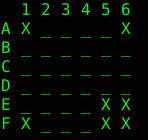
\includegraphics[scale=0.8]{bord_stable.png}
\label{bord_stable}
\caption{Quatre coins du plateau}
\end{figure}

D'autres positions imprenables sont celles qui se retrouvent entre des pions adverses, car ce dernier ne pourra pas non plus les reprendre. Par exemple, dans la FIGURE \ref{exemple_insertion}, on peut voir que le joueur noir (représenté par un 'X') peut effectuer une insertion en jouant en 'A3', le joueur blanc ne pourra pas reprendre ce pion. Au tour suivant, quelque soit le coup du joueur blanc, le joueur noir pourra jouer en 'A1' et ainsi avoir un des coins si désirés, lui permetant ainsi de gagner en stabilité en possédant maintenant trois pions indétronables.

\begin{figure}[H]
\centering
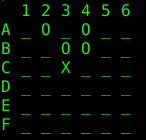
\includegraphics[scale=0.8]{exemple_insertion.png}
\label{exemple_insertion}
\caption{Exemple d'insertion}
\end{figure}

Une autre stratégie reviendrait à diminuer le nombre de coups de l'adversaire tout en augmentant son propre nombre de coups, pour cela on va privilégier les coups rapportant le moins de pions, mais tout en faisant attention à ce que l'adversaire ne puisse pas nous enlever tous nos pions. Réduire le nombre de coups de l'adversaire n'est pas tout, il faut aussi tendre à ne lui laisser la possibilité de ne jouer que des mauvais coups.\\

Comme nous pouvons l'observer à travers les différentes stratégies, nous aurons besoin d'explorer les arbres des coups possibles, mais la complexité d'une telle démarche devient rapidement gigantesque, nous empêchant de parcourir en un temps raisonnable l'arbre en entier. Fort heureusement, nous n'aurons pas besoin de le parcourir en entier, car nous pourrons déterminer que certaines branches de l'arbre ne valent pas le coup d'être explorées.

\subsection{Programmes}

À l'heure actuelle, le programme qui est le champion à ce jeu se nomme Iago. Il se base sur les stratégies énoncées précédemment, mais de part la contrainte technique de temps dûe aux tournois, ils ont dû utiliser certaines astuces. Ainsi, le programme calcule pour chaque coup le temps qu'il peut passer sur celui-ci. Ensuite, durant le temps alloué pour chaque coup, il recherche dans son arbre jusqu'à une profondeur de 7, qu'ils ont jugée comme étant la profondeur donnant le meilleur résultat dans un temps restreint. Pour réduire son temps de réponse, ils ont aussi amélioré les fonctions d'évaluation, mais ils ont surtout réduit le nombre de noeuds que le programme devra examiner.
\newpage

\section{Besoins fonctionnels}

\textbf{Lancer une nouvelle partie de Reversi entre deux utilisateurs :}\\
\begin{itemize}
\item Lancer le programme sans option dans une console de type bash ;
\item Afficher un message de bienvenue et des explications sur le déroulement de la partie (voir \ref{board}) ;\\
\item Initialiser la grille de jeu avec ses dimensions par défaut (voir \ref{board}) ;
\item Déterminer les mouvements possibles pour le joueur en cours ;
\item Mettre à jour la grille de jeu avec les mouvements possibles ;
\item Afficher la grille de jeu ;\\
\item (*) Proposer à l'utilisateur de saisir son mouvement ou de quitter la partie (voir \ref{board}) ;
\item Vérifier que la saisie est valide, retourner à l'étape précédente si ce n'est pas le cas ;\\
\end{itemize}
Si l'utilisateur décide d'un mouvement à réaliser :
\begin{itemize}
\item Vérifier que le mouvement est valide, retourner à l'étape précédente si ce n'est pas le cas ;
\item Mettre à jour la grille de jeu avec le mouvement fraîchement réalisé ;
\item Terminer le tour et changer de joueur ;
\item Déterminer les mouvements possibles pour le joueur en cours;
\item Mettre à jour la grille de jeu avec les mouvements possibles ;
\item Afficher la grille de jeu ;
\item Si la partie se termine, afficher le vainqueur et quitter le programme.
Sinon, retourner à l'étape (*) ;\\
\end{itemize}
Si l'utilisateur décide de quitter la partie :
\begin{itemize}
\item Proposer à l'utilisateur de sauvegarder l'état de la partie en cours avant de quitter (voir \ref{save}) ;
\item Vérifier que la saisie est valide, retourner à l'étape précédente si ce n'est pas le cas ;
\item Si souhaité, sauvegarder l'état de la partie en cours dans un fichier (voir \ref{save}) ;
\item Quitter le programme ;
\end{itemize}
\newpage

\textbf{Lancer une nouvelle partie de Reversi entre l'utilisateur et l'ordinateur :}\\
\begin{itemize}
\item Lancer le programme avec l'option -b ou -w dans une console de type bash (voir \ref{options}) ;
\item Afficher un message de bienvenue et des explications sur le déroulement de la partie (voir \ref{board}) ;\\
\item Initialiser la grille de jeu avec ses dimensions par défaut (voir \ref{board}) ;
\item Déterminer les mouvements possibles pour le joueur en cours ;
\item Mettre à jour la grille de jeu avec les mouvements possibles ;
\item Afficher la grille de jeu ;\\
\end{itemize}
(*) Si c'est au tour de l'utilisateur :
\begin{itemize}
\item Proposer à l'utilisateur de saisir son mouvement ou de quitter la partie (voir \ref{board}) ;
\item Vérifier que la saisie est valide, retourner à l'étape précédente si ce n'est pas le cas ;
\end{itemize}
Si l'utilisateur décide d'un mouvement à réaliser :
\begin{itemize}
\item Vérifier que le mouvement est valide, retourner à l'étape précédente si ce n'est pas le cas ;
\item Mettre à jour la grille de jeu avec le mouvement fraîchement réalisé ;
\item Terminer le tour et changer de joueur ;
\item Déterminer les mouvements possibles pour le joueur en cours ;
\item Mettre à jour la grille de jeu avec les mouvements possibles ;
\item Afficher la grille de jeu ;
\item Si la partie se termine, afficher le vainqueur et quitter le programme.
Sinon, retourner à l'étape (*) ;\\
\end{itemize}
Si l'utilisateur décide de quitter la partie :
\begin{itemize}
\item Proposer à l'utilisateur de sauvegarder l'état de la partie en cours avant de quitter (voir \ref{save}) ;
\item Vérifier que la saisie est valide, retourner à l'étape précédente si ce n'est pas le cas ;
\item Si souhaité, sauvegarder l'état de la partie en cours dans un fichier (voir \ref{save}) ;
\item Quitter le programme ;\\
\end{itemize}
(*) Si c'est au tour de l'ordinateur :
\begin{itemize}
\item Calculer un mouvement à l'aide de la technique d'exploration d'arbre classique choisie ;
\item Mettre à jour la grille de jeu avec le mouvement fraîchement calculé ;
\item Terminer le tour et changer de joueur ;
\item Déterminer les mouvements possibles pour le joueur en cours ;
\item Mettre à jour la grille de jeu avec les mouvements possibles ;
\item Afficher la grille de jeu ;
\item Si la partie se termine, afficher le vainqueur et quitter le programme.
Sinon, retourner à l'étape (*) ;\\
\end{itemize}
\newpage

\textbf{Lancer une nouvelle partie de Reversi entre deux ordinateurs :}\\
\begin{itemize}
\item Lancer le programme avec l'option -a dans une console de type bash (voir \ref{options}) ;
\item Afficher un message de bienvenue et des explications sur le déroulement de la partie (voir \ref{board}) ;\\
\item Initialiser la grille de jeu avec ses dimensions par défaut (voir \ref{board}) ;
\item Déterminer les mouvements possibles pour le joueur en cours ;
\item Mettre à jour la grille de jeu avec les mouvements possibles ;
\item Afficher la grille de jeu ;\\
\item (*) Calculer un mouvement à l'aide de la technique d'exploration d'arbre classique choisie ;
\item Mettre à jour la grille de jeu avec le mouvement fraîchement calculé ;
\item Terminer le tour et changer de joueur ;
\item Déterminer les mouvements possibles pour le joueur en cours ;
\item Mettre à jour la grille de jeu avec les mouvements possibles ;
\item Afficher la grille de jeu ;
\item Si la partie se termine, afficher le vainqueur et quitter le programme.
Sinon, retourner à l'étape (*) ;\\
\end{itemize}

\textbf{Répondre par un mouvement à un état de partie :}
\begin{itemize}
\item Lancer le programme avec l'option -c suivie du nom de fichier contenant l'état de partie dans une console de type bash (voir \ref{options}) ;\\
\item Récupérer le joueur en cours et la grille de jeu à partir des données lues dans le fichier ;
\item Déterminer les mouvements possibles pour le joueur en cours ;
\item Mettre à jour la grille de jeu avec les mouvements possibles ;
\item Afficher la grille de jeu ;\\
\item Calculer un mouvement à l'aide de la technique d'exploration d'arbre classique choisie ;
\item Mettre à jour la grille de jeu avec le mouvement fraîchement calculé ;
\item Terminer le tour et changer de joueur ;
\item Mettre à jour la grille de jeu avec les mouvements possibles ;
\item Afficher la grille de jeu ;
\item Si la partie se termine, afficher le vainqueur et quitter le programme.
Sinon, proposer à l'utilisateur de sauvegarder l'état de la partie en cours avant de quitter (voir \ref{save}) ;
\item Vérifier que la saisie est valide, retourner à l'étape précédente si ce n'est pas le cas ;
\item Si souhaité, sauvegarder l'état de la partie en cours dans un fichier (voir \ref{save}) ;
\item Quitter le programme ;\\
\end{itemize}
\newpage

\textbf{Lancer une partie en modifiant les dimensions de la grille de jeu :}
\begin{itemize}
\item Lancer le programme avec l'option -s suivie d'un entier compris entre 1 et 5 dans une console de type bash (voir \ref{options}) ;
\item Voir les descriptions de parties précédentes ;\\
\end{itemize}

\textbf{Afficher la liste des options disponibles et leurs descriptions :}
\begin{itemize}
\item Lancer le programme avec l'option -h dans une console de type bash (voir \ref{options}) ;
\item Afficher la liste de options disponibles et leurs descriptions ;\\
\end{itemize}

\textbf{Lancer une partie en mode verbeux :}
\begin{itemize}
\item Lancer le programme avec les options voulues ainsi que l'option -v dans une console de type bash (voir \ref{options}) ;
\item Voir les descriptions de parties précédentes, toutes les opérations effectuées seront affichées explicitement ;\\
\end{itemize}

\textbf{Afficher la version du programme :}
\begin{itemize}
\item Lancer le programme avec l'option -V dans une console de type bash (voir \ref{options}) ;
\item Afficher la version du programme ;
\end{itemize}

\subsection{Grille de jeu}
\label{board}

Les cases en abscisses seront numérotées à l'aide de chiffres, les cases en ordonnées seront numérotées à l'aide de lettres (voir figure \ref{exemple_board}). Le joueur pourra alors choisir son mouvement en entrant dans la console la combinaison correspondante à la case souhaitée (exemple : 'A2' ou 'a2').\\

Les cases vides de la grille devront être représentées à l'aide du caractère '\_', le joueur blanc sera représenté par un 'O' et le joueur noir par un 'X'. Les cases où le joueur courant peut effectuer son prochain coup pourront être représentées par '*' (voir FIGURE \ref{exemple_board}). Ce plateau de jeu sera implémenté à l'aide d'une structure de donnée bitboard.

\begin{figure}[H]
\centering
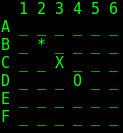
\includegraphics[scale=0.8]{exemple_board.png}
\label{exemple_board}
\caption{Grille initiale}
\end{figure}

\subsection{Sauvegarde}
\label{save}

L'utilisateur peut décider de quitter le jeu et de sauvegarder l'état actuel de la partie en entrant 'Q' (ou 'q') dans la console. Si l'utilisateur décide de quitter le jeu, le programme lui donnera le choix de sauvegarder la partie en cours ou non.En entrant 'Y' (ou 'y'), le programme sauvegardera dans un fichier le tour du joueur courant ('X' ou 'O') ainsi que l'état de la grille actuelle. Le fichier sera présenté de la même manière que le jeu, mais sans la numérotation des cases ni les mouvements possibles (représentés avec le caractère '*') (voir FIGURE \ref{exemple_save}). Le format de sortie pour le fichier de sauvegarde doit être \textit{.txt}. Si le joueur entre 'N' (ou 'n'), le programme ne sauvegardera pas le plateau.

\begin{figure}[H]
\centering
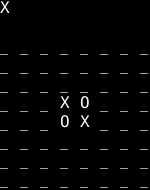
\includegraphics[scale=0.8]{exemple_save.png}
\label{exemple_save}
\caption{Sauvegarde grille initiale}
\end{figure}

\subsection{Options}
\label{options}

Au lancement du programme, l'utilisateur devra pouvoir modifier certains paramètres de la partie grâce à des options :\\
\begin{itemize}
\item [-c, --contest] : Permet de démarrer le programme en mode compétition. Cette option prend en entrée un fichier contenant la sauvegarde d'un jeu et joue le coup suivant.
\item [-s, --size] : Permet de démarrer le programme en ayant modifié la taille du plateau de jeu. Cette option prend en entrée un entier compris entre 1 et 5, ce qui permet de faire varier la taille du plateau de 2 à 10 cases.
\item [-b, --black-ai] : Permet de démarrer le programme en ayant spécifié que l'ordinateur jouera pendant la partie et contrôlera les noirs.
\item [-w, --white-ai] : Permet de démarrer le programme en ayant spécifié que l'ordinateur jouera pendant la partie et contrôlera les blancs.
\item [-a, --all-ai] : Permet de démarrer le programme en ayant spécifié que l'ordinateur jouera la partie, il contrôlera les noirs et les blancs.
\item [-h, --help] : Permet d'afficher la liste des options et leurs descriptions.
\item [-v, --verbose]: Permet de démarrer le programme en mode verbeux.
\item [-V, --version]: Permet d'afficher la version du programme.
\end{itemize}
\newpage

\section{Besoins non fonctionnels}

\begin{itemize} 
\item Rapidité d'exécution : chaque coup doit être exécuté en moins d'une seconde.
\item Portabilité : le programme doit pouvoir s'exécuter indépendamment de la machine, du système d'exploitation et de ses configurations.
\item Confiance : les règles doivent être respectées et les fichiers de sauvegarde doivent suivre le format et la forme attendue (voir \ref{save}).
\end{itemize}

\section{Diagrammes techniques}

\subsection{Diagramme de cas d'utilisation}

\begin{figure}[H]
\centering
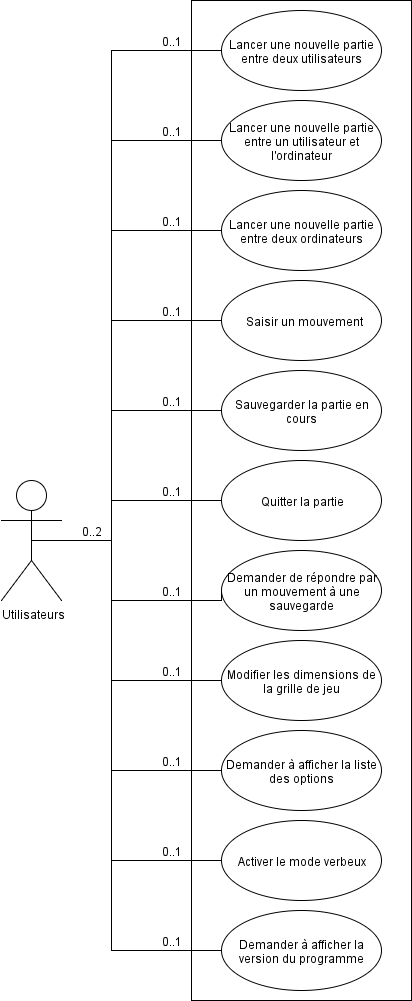
\includegraphics[scale=0.5]{use_case.png}
\label{use_case}
\caption{Diagramme de cas d'utilisation}
\end{figure}


\end{document}